\scanpage{3}
Chirurgie des surfaces conformes.

1) \uline{Découpage} : \unsure{Découpe} d'une surface conforme \deleted{\unsure{sans bord}} (\unsure{évt}
avec bord) suivant un sous-1-complexe rectifiable
compact : On trouve une surface conforme à \deleted{\unsure{un}}
bord, avec morceau \inserted{\deleted{compact}} de bord compact marqué

2) \uline{Recollage} : À partir d'une surface conforme
(avec bord \deleted{\unsure{si on veut}}) et d'un morceau
compact du bord, et une relation d'équivalence
``admissible'' \inserted{(au sens rectifiable)} sur le bord, \deleted{\unsure{on a}} on trouve
une surface conforme avec bord\ldots

3) \uline{\unsure{Rétrécissage}}
\[
\underset{\substack{1\text{-compl.}\\\text{cpt}}}{K}
\subset
\underset{\text{s. conforme avec bord}\ \unsure{?}}{X}
\]
$\widetilde X$ découpé de $X$ suivant $K$, $\partial'\widetilde X$ partie distinguée
du bord, on choisit un \inserted{multi-}anneau autour de
$\partial'\widetilde X$, \deleted{\unsure{soit alors}} (un germe
de \unsure{tel anneau} autour
d'une composante
$(\partial'_{\unsure{i}}\widetilde X)_{\unsure{i}}$ \unsure{revient} : la donnée
d'une structure Riemannienne
\deleted{régulière} \inserted{rectifiable} de long. totale $1$
sur celle-ci\ldots)

\figure{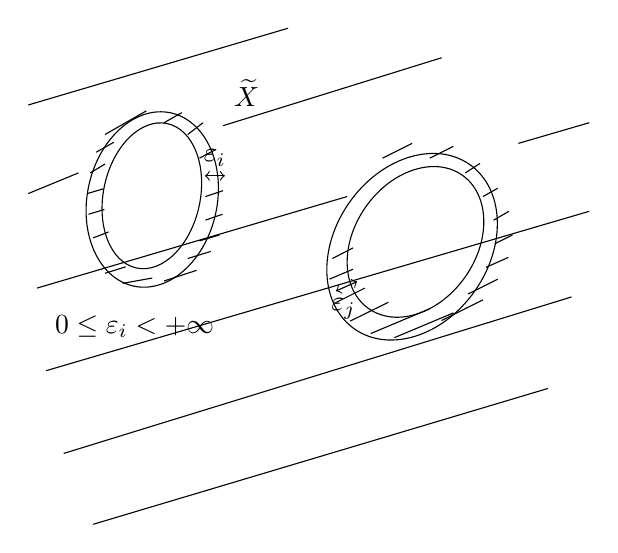
\begin{tikzpicture}[x=0.75cm,y=0.75cm]
\draw (-.3,2.8)--(4.1,4.1);
\draw (-.3,1.3)--(.55,1.65) (3.0,2.45)--(6.7,3.6);
\draw (-.15,-.3)--(5.1,1.25) (8.0,2.15)--(9.2,2.5);
\draw (0,-1.7)--(9.2,1.0);
\draw (.3,-3.1)--(8.9,-.45);
\draw (.8,-4.3)--(8.5,-2.0);
\draw[rotate around={-12:(1.8,1.2)}] (1.8,1.2) ellipse (1.1 and 1.5);
\draw[rotate around={-12:(1.8,1.2)}] (1.78,1.26) ellipse (.82 and 1.25);
\draw (1.0,2.3)--(1.7,2.7) (.85,2.0)--(1.15,2.17) (.75,1.65)--(1,1.8)
(.7,1.3)--(.97,1.38) (.72,.95)--(.99,1.03) (.8,.55)--(1.06,.65)
(1,-.05)--(1.35,.06) (1.3,-.22)--(1.8,-.13) (2,-.18)--(2.55,0)
(2.4,.2)--(2.79,.32) (2.6,.5)--(2.94,.6) (2.7,.85)--(2.99,.95)
(2.7,1.25)--(3,1.35) (2.6,1.9)--(2.88,2.05) (2.4,2.3)--(2.66,2.5)
(2.0,2.5)--(2.3,2.67);
\draw[rotate around={-35:(6.2,.4)}] (6.2,.4) ellipse (1.3 and 1.7);
\draw[rotate around={-35:(6.2,.4)}] (6.2,.5) ellipse (1.03 and 1.38);
\draw (4.85,.2)--(5.2,.38) (4.8,-.15)--(5.2,.02) (4.9,-.55)--(5.4,-.3)
(5.15,-.86)--(5.8,-.54) (5.5,-1.07)--(6.5,-.65) (5.9,-1.14)--(6.9,-.72)
(6.7,-.85)--(7.4,-.5) (7.15,-.4)--(7.65,-.15) (7.45,.05)--(7.83,.22)
(7.6,.45)--(7.9,.6) (7.58,.85)--(7.84,1.0) (7.4,1.25)--(7.65,1.39)
(7.1,1.65)--(7.35,1.81) (6.5,1.9)--(6.9,2.1) (5.7,1.9)--(6.2,2.15);
\node at (3.4,3.0) {$\widetilde X$};
\draw[<->] (2.69,1.6)--(3.03,1.6);
\node[above] at (2.86,1.6) {$\varepsilon_{\unsure{i}}$};
\draw[<->] (4.91,-.35)--(5.27,-.19);
\node[below] at (5.04,-.32) {$\varepsilon_{\unsure{j}}$};
\node at (1.5,-.95) {$0\leq\varepsilon_i<+\infty$};
\end{tikzpicture}}

$\widetilde X^*$ la surface \inserted{\deleted{à bord \unsure{droit}}\inserted{\unsure{droit}}\deleted{\unsure{rectif.}}} rétrécie
\unsure{déduit} de la couronne
choisissons un isomorphisme rectifiable
$\partial'\widetilde X^*\xrightarrow{\sim}\partial'\widetilde X$ compatible avec les comp. connexes,
et utilisons la relation d'équivalence \inserted{de recollage} sur
$\partial'\widetilde X$ pour en déduire une sur $\widetilde X^*$. On
en \unsure{conclut} \deleted{$\unsure{K\subset}$} $X^*$ et $K\subset X^*$
% archive foliation: 2
